\section{\xxx Overview} \label{sec:overview}

Figure 2 shows \xxx's architecture. It contains two main components: 
the Serviceguard and the protocol. 

The protocol component interposes on \tapsend on receiving a network packet 
and runs a RDMA-based consensus process on this request. Besides, this component 
maintains a packet queue to capture outgoing packets by interposing on 
\taprecv and invokes the output checking protocol periodically. 

The Serviceguard component monitors the overall health of the configured applications. 
It sends the application heartbeat to the protocol component in the physical 
host. The Serviceguard uses the application heartbeat as the communication 
medium to convey the status of the application to the protocol component. 
In addition, the Serviceguard is also responsible for checkpoint and restore. 

% On receiving a packet, QEMU calls tap_send()
% On sending a packet, QEMU calls tap_receive()
% We maintain a packet queue to capture outgoing packets.

\begin{figure}[t]
% \vspace{.20in}
\centering
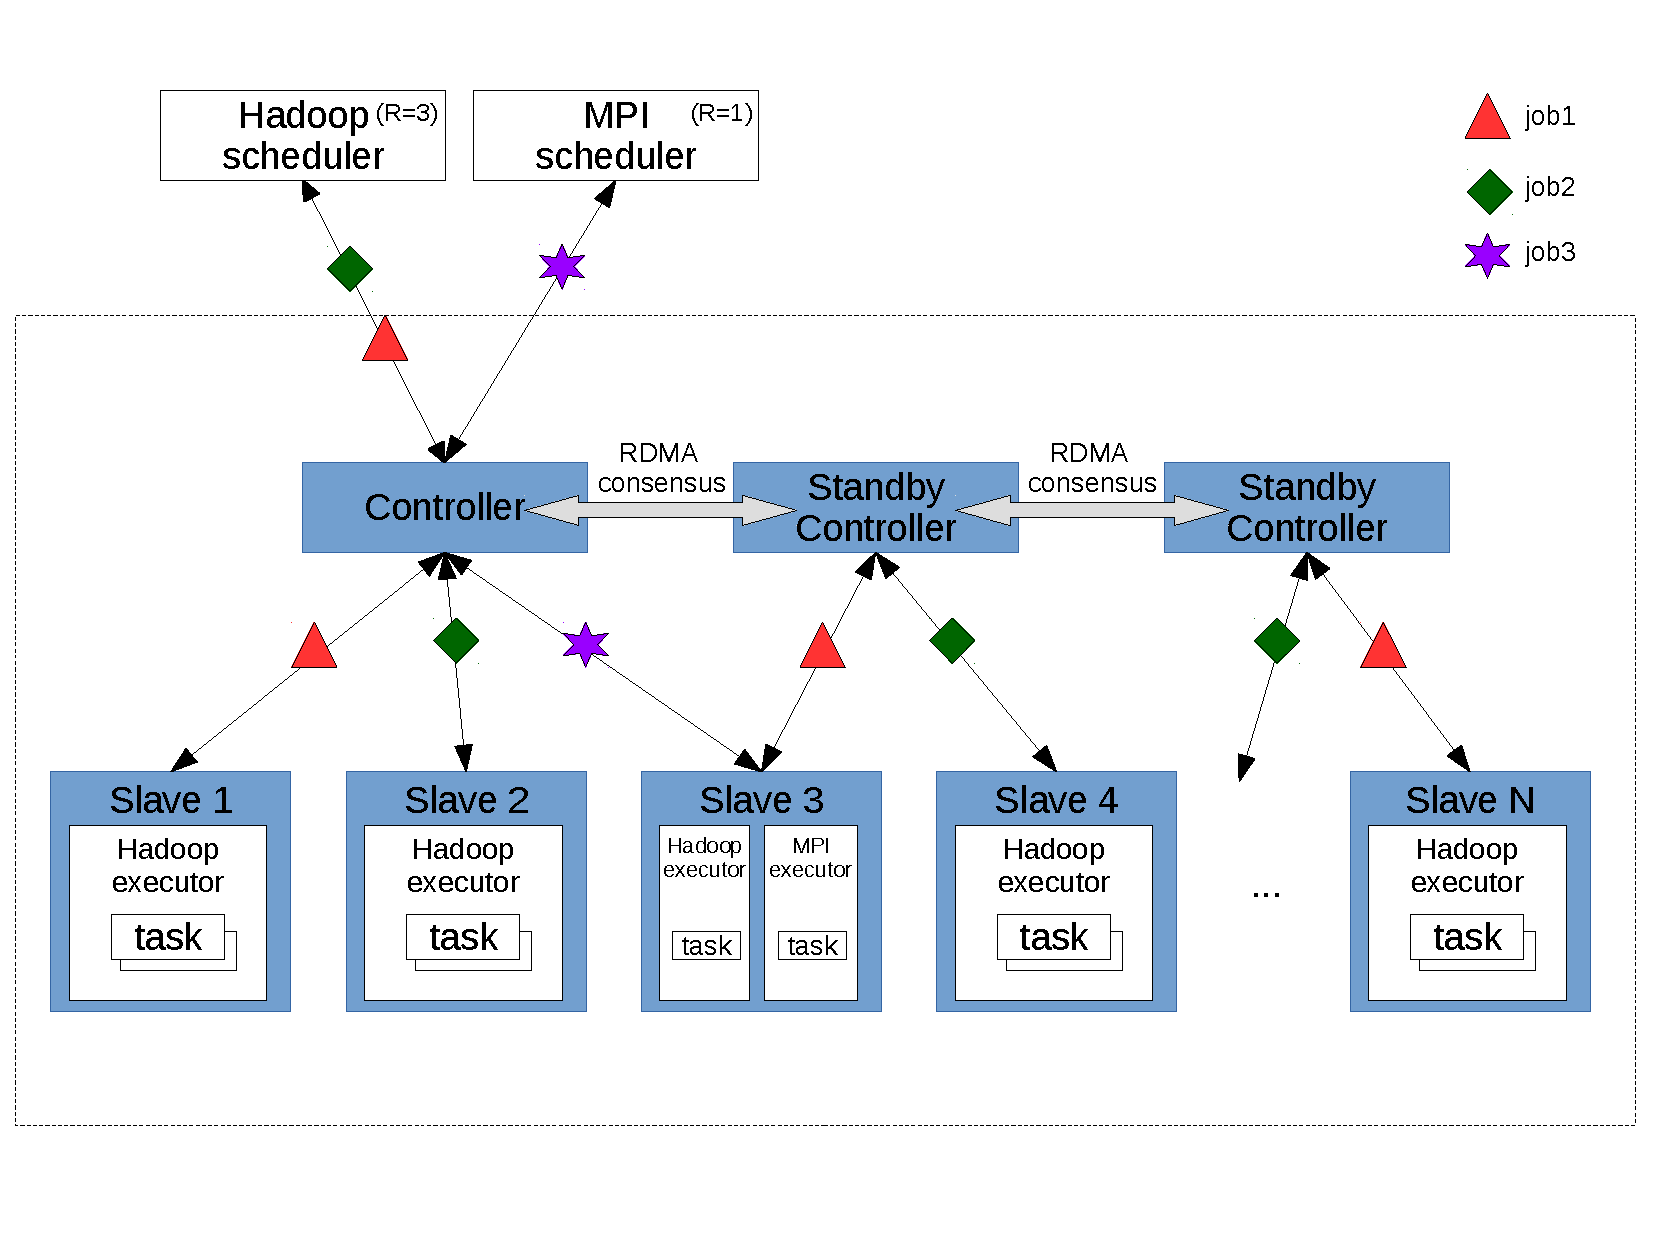
\includegraphics[width=.47\textwidth]{figures/arch}
\vspace{-.2in}
\caption{{\em The \xxx Architecture.} Key components are shaded (and
in blue).} \label{fig:arc}
\vspace{.05in}
\end{figure}
